\documentclass{beamer}
\usepackage[utf8]{inputenc}

\usepackage{amsmath}
\usepackage{semantic}
\usepackage{graphicx}
\usepackage{booktabs}
%\usepackage{todonotes}
\usepackage[absolute,overlay]{textpos}
\usepackage{tikz}
\usetikzlibrary{matrix,positioning,arrows}

\tikzset{
mymat/.style={
  matrix of math nodes,
  text height=2.5ex,
  text depth=0.75ex,
  text width=3.25ex,
  align=center,
  column sep=-\pgflinewidth
  }
}


\mode<presentation> {
\usetheme{boxes} % When headline is wanted use Dresden theme instead
\usecolortheme{seagull}
\setbeamertemplate{footline}[page number]
\setbeamertemplate{navigation symbols}{}
}

\newcommand{\kw}[1]{\texttt{#1}}
\newcommand{\lvl}[1]{\langle #1 \rangle}
\newcommand{\push}[2]{[ #1 ] \lvl{#2}}
\newcommand{\backupbegin}{
   \newcounter{finalframe}
   \setcounter{finalframe}{\value{framenumber}}
}

\newcommand{\backupend}{
   \setcounter{framenumber}{\value{finalframe}}
}

%----------------------------------------------------------------------------------------
%	TITLE PAGE
%----------------------------------------------------------------------------------------

\title[FCL] % bottom of every slide
  {FCL: A low-level functional GPU language} % title page

\subtitle{(Work in progress)}

\author{\footnotesize{Martin Dybdal} \\ \footnotesize{\texttt{dybber@dybber.dk}}}

\institute {
DIKU \\
University of Copenhagen
}

% \title[Group Theory]{A longer title of the talk concerning Group Theory}
% \author[short name]{My full name}
% \institute[My Inst.]{Full Institut Name}
% % logo of my university

\date[7 July 2016]{7 July 2016}

\begin{document}

{
\setbeamertemplate{headline}{}
\begin{frame}
  \titlepage

  \begin{center} {\small Joint work w. Mary Sheeran, Joel Svensson and
      Martin Elsman}
  \end{center}


  \note{I started thinking during master thesis, ~ 3 years
    ago. decided to start top down.}
\end{frame}
}

%----------------------------------------------------------------------------------------
%	TABLE OF CONTENTS
%----------------------------------------------------------------------------------------

% \begin{frame}
% \frametitle{Overview}
% \tableofcontents
% \end{frame}

%----------------------------------------------------------------------------------------
%	CONTENT
%----------------------------------------------------------------------------------------


\section{Overview}

% \begin{frame}[fragile]

%   \begin{itemize}
%   \item Introduction
%     \begin{itemize}
%     \item Why a low-level composable GPU language?
%     \item Get a feel for FCL, example: reverse
%     \end{itemize}
%   \item FCL by example: transpose
%     \begin{itemize}
%     \item Graphic illustration
%     \item Idea one: Pull array vs. push array
%     \item Idea two: Nested arrays, but only non-nested arrays can be materialized
%     \item Level hierarchy
%     \item Use of shared-memory
%     \item \texttt{force} is the key primitive
%     \item Show OpenCL code
%     \end{itemize}
%   \item FCL by example: reduction
%     \begin{itemize}
%     \item Hierarchy polymorphism
%     \item Show OpenCL code
%     \end{itemize}
%   \item Performance results
%   \item Formalism highlights
%   \item Future work
%     \begin{itemize}
%     \item manual memory management
%     \item sequential loops
%     \item multidimensional arrays
%     \item tracking communication costs
%     \end{itemize}
%   \item Key messages
%   \end{itemize}

% \end{frame}

% \begin{frame}
%   TODOs

%   \begin{itemize}
%   \item Something on Fusion
%   \item Slides on formalisation
%   \item Take-home messages slide
%   \end{itemize}
% \end{frame}

\begin{frame}[fragile]
  \frametitle{Agenda}

\begin{itemize}
\item Why a new low-level language for GPU computing?
\item FCL by example
\item Performance results
\item Formalising FCL (just the highlights)
\item Future work
\end{itemize}
\end{frame}

\begin{frame}
\frametitle{Why a new low-level language for GPU computing?}
\begin{itemize}
\item Composability and agility
\item Built in fusion, user-controlled
\item Compare programs/algorithms
\item Predictability, no black box wrt. performance
\item Ability to optimize
\item A quest for a GPU language for algorithms researchers
\item Intermediate language for optimizing compilers
\end{itemize}
\end{frame}

\begin{frame}[fragile]
\frametitle{Reverse: A simple example}

\begin{verbatim}
sig reverse : [a] -> [a]
fun reverse arr =
  let n = length arr
  in generate n (fn i => index arr (n - i - 1))
\end{verbatim}

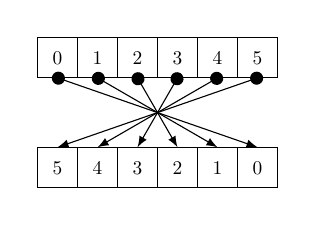
\begin{tikzpicture}[>=latex, scale=0.7, every node/.style={scale=0.7}]
\matrix[mymat, anchor=west,style={nodes=draw}]
at (0,0) 
(mat1)
{
0 & 1 & 2 & 3 & 4 & 5 \\
};
\matrix[mymat,anchor=west, style={nodes=draw}]
at (0,-2)
(mat2)
{
5 & 4 & 3 & 2 & 1 & 0 \\
};

\begin{scope}[shorten <= -2pt]
\draw[*->]
  (mat1-1-1.south) -- (mat2-1-6.north);
\draw[*->]
  (mat1-1-2.south) -- (mat2-1-5.north);
\draw[*->]
  (mat1-1-3.south) -- (mat2-1-4.north);
\draw[*->]
  (mat1-1-4.south) -- (mat2-1-3.north);
\draw[*->]
  (mat1-1-5.south) -- (mat2-1-2.north);
\draw[*->]
  (mat1-1-6.south) -- (mat2-1-1.north);
\end{scope}
\end{tikzpicture}


\pause

How is this executed on a GPU?
\begin{itemize}
\item Sequential in a single thread?
\item Performed in a single block?
\item Performed among threads in a grid?
\end{itemize}

\end{frame}

\begin{frame}[fragile]
\frametitle{Reverse: Distributed}

{\small
\begin{verbatim}
sig revBlock : [a] -> [a]<block>
fun revBlock arr = push <block> (reverse arr)

sig revDistribute : int -> [a] -> [a]<grid>
fun revDistribute chunkSize arr =
  splitUp chunkSize arr
   |> map reverseBlock
   |> reverse
   |> concat chunkSize
\end{verbatim}
}

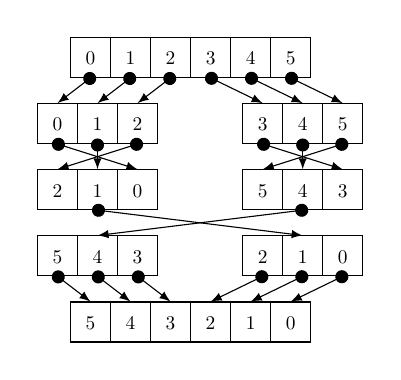
\begin{tikzpicture}[>=latex, scale=0.7, every node/.style={scale=0.7}]
\matrix[mymat, anchor=west,style={nodes=draw}]
at (0.6,0) 
(mat1)
{
0 & 1 & 2 & 3 & 4 & 5 \\
};

\matrix[mymat, anchor=west,style={nodes=draw}]
at (0,-1.2) 
(mat21)
{
0 & 1 & 2 \\
};

\matrix[mymat, anchor=west,style={nodes=draw},right of=mat21]
at (4,-1.2) 
(mat22)
{
3 & 4 & 5 \\
};

\matrix[mymat, anchor=west,style={nodes=draw}]
at (0,-2.4) 
(mat31)
{
2 & 1 & 0 \\
};

\matrix[mymat, anchor=west,style={nodes=draw},right of=mat31]
at (4,-2.4) 
(mat32)
{
5 & 4 & 3 \\
};


\matrix[mymat, anchor=west,style={nodes=draw}]
at (0,-3.6) 
(mat41)
{
5 & 4 & 3 \\
};

\matrix[mymat, anchor=west,style={nodes=draw}, right of=mat41]
at (4,-3.6) 
(mat42)
{
2 & 1 & 0 \\
};

\matrix[mymat,anchor=west, style={nodes=draw}]
at (0.6,-4.8)
(mat5)
{
5 & 4 & 3 & 2 & 1 & 0 \\
};
\begin{scope}[shorten <= -2pt]
\draw[*->]
  (mat1-1-1.south) -- (mat21-1-1.north);
\draw[*->]
  (mat1-1-2.south) -- (mat21-1-2.north);
\draw[*->]
  (mat1-1-3.south) -- (mat21-1-3.north);
\draw[*->]
  (mat1-1-4.south) -- (mat22-1-1.north);
\draw[*->]
  (mat1-1-5.south) -- (mat22-1-2.north);
\draw[*->]
  (mat1-1-6.south) -- (mat22-1-3.north);

\draw[*->]
  (mat21-1-1.south) -- (mat31-1-3.north);
\draw[*->]
  (mat21-1-2.south) -- (mat31-1-2.north);
\draw[*->]
  (mat21-1-3.south) -- (mat31-1-1.north);
\draw[*->]
  (mat22-1-1.south) -- (mat32-1-3.north);
\draw[*->]
  (mat22-1-2.south) -- (mat32-1-2.north);
\draw[*->]
  (mat22-1-3.south) -- (mat32-1-1.north);

\draw[*->]
  (mat31-1-2.south) -- (mat42-1-2.north);
\draw[*->]
  (mat32-1-2.south) -- (mat41-1-2.north);


\draw[*->]
  (mat41-1-1.south) -- (mat5-1-1.north);
\draw[*->]
  (mat41-1-2.south) -- (mat5-1-2.north);
\draw[*->]
  (mat41-1-3.south) -- (mat5-1-3.north);
\draw[*->]
  (mat42-1-1.south) -- (mat5-1-4.north);
\draw[*->]
  (mat42-1-2.south) -- (mat5-1-5.north);
\draw[*->]
  (mat42-1-3.south) -- (mat5-1-6.north);
\end{scope}
\end{tikzpicture}
\end{frame}

\begin{frame}[fragile]
  \frametitle{Reverse: Generated OpenCL}
\begin{verbatim}
sig revKernel : [int] -> [int]<grid>
kernel revKernel arr = revDistribute #BlockSize arr
  config #BlockSize = 256
\end{verbatim}

~

{\tiny
  \begin{verbatim}
__kernel void revKernel(__global int* arrInput_0, int lenInput_1,
                        __global int* arrOutput_3) {
    int n_2 = lenInput_1 / 256;
    int blocksQ_5 = n_2 / get_num_groups(0);
    for (int i_6 = 0; i_6 < blocksQ_5; i_6++) {
        int j_8 = (get_group_id(0) * blocksQ_5) + i_6;
        arrOutput_3[((j_8 * 256) + get_local_id(0))] = 
            arrInput_0 [((((n_2 - j_8) - 1) * 256) + ((256 - get_local_id(0)) - 1))];
        barrier(CLK_LOCAL_MEM_FENCE);
    }
    if (get_group_id(0) < (n_2 % get_num_groups(0))) {
        int j_16 = (get_num_groups(0) * blocksQ_5) + get_group_id(0);
        arrOutput_3[((j_16 * 256) + get_local_id(0))] = 
            arrInput_0 [((((n_2 - j_16) - 1) * 256) + ((256 - get_local_id(0)) - 1))];
        barrier(CLK_LOCAL_MEM_FENCE);
    }
}
\end{verbatim}
}
\end{frame}

\begin{frame}[fragile,fragile]
  \frametitle{Two array types}
  \framesubtitle{(from Obsidian)}

  \begin{itemize}
  \item Pull arrays: for organizing computation, indexable no concatenation
    \begin{verbatim}
       [int], [bool], [[int]]\end{verbatim}
  \item Push arrays: for writing to memory, non indexable, supports concatenation
    \begin{verbatim}
       [int]<thread>, [int]<block>, [int]<grid>\end{verbatim}
   \item Both supporting fusion
  \end{itemize}  
\end{frame}

\begin{frame}[fragile]
  \frametitle{Array types in reverse}
\begin{verbatim}
sig revDistribute : int -> [a] -> [a]<grid>
fun revDistribute chunkSize arr =
  splitUp chunkSize arr    -- [[a]]
   |> map reverseBlock     -- [[a]<block>]
   |> reverse              -- [[a]<block>]
   |> concat chunkSize     -- [a]<grid>

sig push : <lvl> -> [a] -> [a]<lvl>
sig splitUp : int -> [a] -> [[a]]
sig concat : int -> [[a]<lvl>] -> [a]<1+lvl>
\end{verbatim}

\end{frame}

\begin{frame}[fragile]
  \frametitle{Matrix transposition}
  \framesubtitle{A basic approach}

\begin{verbatim}
sig transpose : int -> int -> [a] -> [a]
fun transpose cols rows elems =
  generate (cols * rows)
           (fn n =>
              let i = n / rows in
              let j = n % rows
              in index elems (j * rows + i))
\end{verbatim}

\end{frame}

\begin{frame}[fragile]
  \frametitle{Matrix transposition}
  \framesubtitle{Tiled}

\includegraphics[width=\textwidth]{../sharedTranspose-1024x409.jpg}

\quad(Figure by NVIDIA)
\end{frame}


\begin{frame}[fragile]
  \frametitle{Matrix transposition}
  \framesubtitle{Tiled}

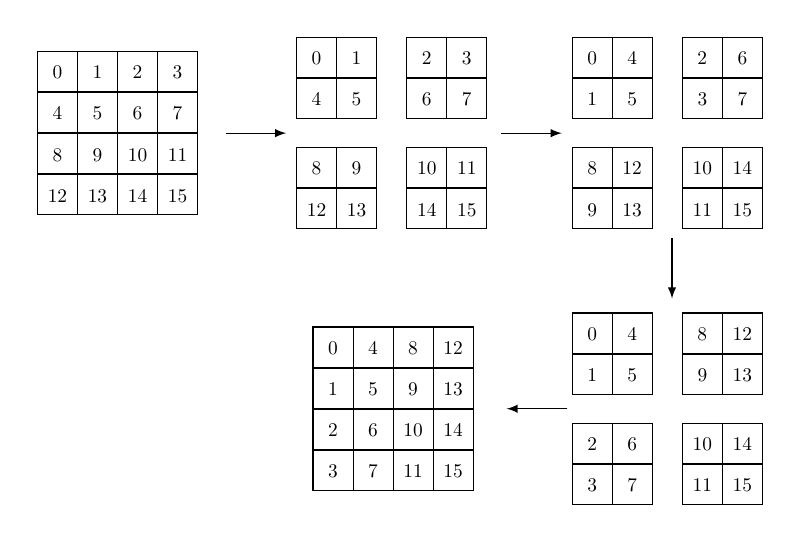
\begin{tikzpicture}[>=latex, scale=0.7, every node/.style={scale=0.7}]
\matrix[mymat, anchor=west,style={nodes=draw}]
at (0.3,0) 
(mat1)
{
0 & 1 & 2 & 3 \\
4 & 5 & 6 & 7 \\
8 & 9 & 10 & 11 \\
12 & 13 & 14 & 15 \\
};
\matrix[mymat, anchor=west,style={nodes=draw}]
at (5,1) 
(mat21)
{
0 & 1 \\
4 & 5 \\
};
\matrix[mymat, anchor=west,style={nodes=draw}]
at (7,1) 
(mat22)
{
2 & 3 \\
6 & 7 \\
};
\matrix[mymat, anchor=west,style={nodes=draw}]
at (5,-1) 
(mat23)
{
8 & 9 \\
12 & 13 \\
};
\matrix[mymat, anchor=west,style={nodes=draw}]
at (7,-1) 
(mat24)
{
10 & 11 \\
14 & 15 \\
};

\matrix[mymat, anchor=west,style={nodes=draw}]
at (10,1) 
(mat31)
{
0 & 4 \\
1 & 5 \\
};
\matrix[mymat, anchor=west,style={nodes=draw}]
at (12,1) 
(mat32)
{
2 & 6 \\
3 & 7 \\
};
\matrix[mymat, anchor=west,style={nodes=draw}]
at (10,-1) 
(mat33)
{
8 & 12 \\
9 & 13 \\
};
\matrix[mymat, anchor=west,style={nodes=draw}]
at (12,-1) 
(mat34)
{
10 & 14 \\
11 & 15 \\
};


\matrix[mymat, anchor=west,style={nodes=draw}]
at (10,-4) 
(mat41)
{
0 & 4 \\
1 & 5 \\
};
\matrix[mymat, anchor=west,style={nodes=draw}]
at (12,-4) 
(mat42)
{
8 & 12 \\
9 & 13 \\
};
\matrix[mymat, anchor=west,style={nodes=draw}]
at (10,-6) 
(mat43)
{
2 & 6 \\
3 & 7 \\
};
\matrix[mymat, anchor=west,style={nodes=draw}]
at (12,-6) 
(mat44)
{
10 & 14 \\
11 & 15 \\
};

\matrix[mymat, anchor=west,style={nodes=draw}]
at (5.3,-5) 
(mat5)
{
0 & 4 & 8 & 12 \\
1 & 5 & 9 & 13 \\
2 & 6 & 10 & 14 \\
3 & 7 & 11 & 15 \\
};

\begin{scope}[shorten <= -2pt]
\draw[->]
  (4,0) -- (5,0);
\draw[->]
  (9,0) -- (10,0);
\draw[->]
  (12,-2) -- (12,-3);
\draw[->]
  (10,-5) -- (9,-5);
\end{scope}
\end{tikzpicture}
\end{frame}



\begin{frame}[fragile,fragile]
\frametitle{Matrix transposition}
\framesubtitle{Tiled, using shared-memory}

{\small
\begin{verbatim}
sig transposeTiled : int -> int -> int -> [a] -> [a]<grid>
fun transposeTiled tileDim cols rows mat =
  let n = cols / tileDim
      m = rows / tileDim
  in split2DGrid tileDim cols n m mat
       |> map (force . push <block>)
       |> map (transpose tileDim tileDim)
       |> transpose n m
       |> map (push <block>)
       |> concat2DGrid tileDim n rows
\end{verbatim}
}

\begin{verbatim}
sig force : [a]<lvl> -> [a]
\end{verbatim}

\end{frame}

\begin{frame}
  \frametitle{Performance}
  \includegraphics[width=\textwidth]{../bandwidth}

  NVIDIA GeForce GTX 780 Ti (2880 cores, 875 Mhz, 3GB GDDR5)
  
  Peak bandwidth 254.90 GB/s (measured)
\end{frame}

\begin{frame}
  \frametitle{Highlights from formalism}

  \begin{itemize}
  \item Polymorphic type system, restricting e.g. the valid nesting of arrays
  \item Dynamic semantics, explaining mapping to threads, blocks, warps and grids
  \item Formalism informed our implementation
  \item Abstracts away from block/warp-virtualization
  \item Classic type safety properties
  \end{itemize}

\end{frame}

\begin{frame}
  \frametitle{Built-in operators}

  \begin{align*}
      \kw{lengthPull} :~& [\alpha] -> \kw{int} \\
     \kw{lengthPush} :~& \push{\alpha}{lvl} -> \kw{int} \\
     \kw{mapPull} :~& (\alpha -> \beta) -> [\alpha] -> [\beta] \\
     \kw{mapPush} :~& (\alpha -> \beta) -> \push{\alpha}{lvl} -> \push{\beta}{lvl} \\
     \\
     \kw{generate} :~& \kw{int} -> (\kw{int} -> \alpha) -> [\alpha] \\
     \kw{index} :~& [\alpha] -> \kw{int} -> \alpha \\
     \\
     \kw{push} :~& \lvl{lvl} -> [\alpha] -> \push{\alpha}{lvl} \\
     \kw{force} :~& \push{\alpha}{lvl} -> [\alpha] \\
     \kw{concat} :~& \kw{int} -> [\push{\alpha}{lvl}] -> \push{\alpha}{1+lvl} \\
     \\
     \kw{while} :~& ([\alpha] -> \kw{bool}) -> ([\alpha] -> \push{\alpha}{lvl}) -> \push{\alpha}{lvl} -> [\alpha]
%     % \kw{interleave} :~& \kw{int} -> (\kw{int} -> \kw{int} -> \kw{int}) -> [\push{\alpha}{lvl}] -> \push{\alpha}{1+lvl} \\
  \end{align*}
\end{frame}



\begin{frame}
  \frametitle{Future work on FCL}
  \begin{itemize}
  \item Multi-dimensional arrays
  \item Tracking communication costs in semantics
  \item Generalize hierarchy and mapping \\
    {\small (e.g. ability to add layers, like multiple GPUs)}
  \end{itemize}
\end{frame}

\begin{frame}
\frametitle{Summary}

\begin{itemize}
\item I argue that we need to focus on performance reasoning and
  cost-models
\item Nested arrays, but only non-nested arrays can be materialized.
\item Level hierarchy controls mapping to sequential/parallel loops
\item FCL is very much work in progress
\end{itemize}

\end{frame}

\begin{frame}
\frametitle{References}
\footnotesize{
\begin{thebibliography}{99} % Beamer does not support BibTeX so references must be inserted manually as below
\bibitem{p1} Obsidian: A domain specific embedded language for parallel programming of graphics processor
\newblock Joel Svensson, Mary Sheeran, Koen Claessen, 2011
\newblock \emph{IFL'11}

\bibitem{p2} Compiling a Subset of APL Into a Typed Intermediate Language.
\newblock Martin Elsman and Martin Dybdal, 2014
\newblock \emph{ARRAY'14}
\end{thebibliography}
}
\end{frame}

\begin{frame}
\frametitle{Thank you}

Martin Dybdal \\
Ph.D. student \\
DIKU, University of Copenhagen \\
\texttt{dybber@dybber.dk} \\
%\texttt{@martindybdal}\\
~\\
FCL is available at: \url{http://github.com/dybber/fcl}
\end{frame}

\appendix
\backupbegin

\begin{frame}
  \frametitle{More future work on FCL}

  \begin{itemize}
  \item Manual memory-management
  \item Sequential loops
  \item Larger examples
  \item Host-code generation
  \item Use as backend for our APL-compiler (TAIL)
  \end{itemize}
\end{frame}

\begin{frame}[fragile]
  \frametitle{Reduction}
\begin{verbatim}
sig halve : [a] -> ([a], [a])
sig zipWith : (a -> b -> c) -> [a] -> [b] -> [c]

sig step : <lvl> -> (a -> a -> a) -> [a] -> [a]<lvl>
fun step <lvl> f arr =
  let x = halve arr
  in push <lvl> (zipWith f (fst x) (snd x))
\end{verbatim}

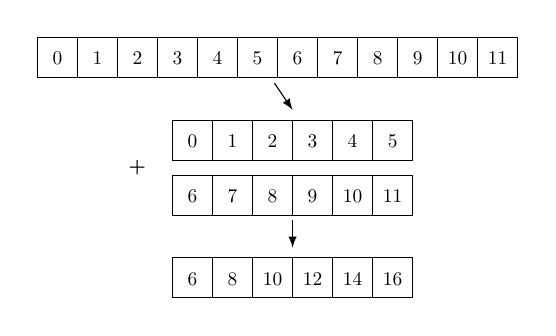
\begin{tikzpicture}[>=latex, scale=0.7, every node/.style={scale=0.7}]
\matrix[mymat, anchor=west,style={nodes=draw}]
at (0,0) 
(mat1)
{
0 & 1 & 2 & 3 & 4 & 5 & 6 & 7 & 8 & 9 & 10 & 11\\
};
\matrix[mymat,anchor=west, style={nodes=draw}]
at (2.45,-1.5)
(mat2)
{
0 & 1 & 2 & 3 & 4 & 5 \\
};
\matrix[mymat,anchor=west, style={nodes=draw}]
at (2.45,-2.5)
(mat3)
{
6 & 7 & 8 & 9 & 10 & 11\\
};

\matrix[mymat,anchor=west, style={nodes=draw}]
at (2.45,-4)
(mat4)
{
6 & 8 & 10 & 12 & 14 & 16\\
};

\node at (2,-2)
  (addsymb) {\bf +};

\begin{scope}[shorten <= -2pt]
\draw[->]
  (mat1.south) -- (mat2.north);
\draw[->]
  (mat3.south) -- (mat4.north);
\end{scope}
\end{tikzpicture}


\end{frame}

\begin{frame}[fragile]
  \frametitle{Reduction}
  \begin{verbatim}
sig red : <lvl> -> (a -> a -> a) -> [a] -> [a]<lvl>
fun red <lvl> f arr =
  while (fn arr => 1 != lengthPull arr)
        (step <lvl> f)
        (step <lvl> f arr)
  |> push <lvl>
\end{verbatim}
\end{frame}

\begin{frame}[fragile]
  \frametitle{Reduction}
  \framesubtitle{OpenCL}

{\tiny
\begin{verbatim}
__kernel void reduceAdd(__local volatile uchar* sbase,
                        __global int* arrInput_0, int lenInput_1,
                        __global int* arrOutput_2) {
    int ub_3 = lenInput_1 >> 8;
    int blocksQ_4 = ub_3 / get_num_groups(0);
    for (int i_5 = 0; i_5 < blocksQ_4; i_5++) {
        int j_7 = (get_group_id(0) * blocksQ_4) + i_5;
        __local volatile int* arr_12 = (__local volatile int*) (sbase + 0);
        arr_12[get_local_id(0)] = arrInput_0 [((j_7 * 256) + get_local_id(0))]
                                + arrInput_0 [((j_7 * 256) + (get_local_id(0) + 128))];
        barrier(CLK_LOCAL_MEM_FENCE);
        if (get_local_id(0) < 64) {
            arr_12[get_local_id(0)] = arr_12 [get_local_id(0)] + arr_12 [(get_local_id(0) + 64)];
        }
        barrier(CLK_LOCAL_MEM_FENCE);
        if (get_local_id(0) < 32) {
            arr_12[get_local_id(0)] = arr_12 [get_local_id(0)] + arr_12 [(get_local_id(0) + 32)];
        }
        barrier(CLK_LOCAL_MEM_FENCE);
        if (get_local_id(0) < 16) {
            arr_12[get_local_id(0)] = arr_12 [get_local_id(0)] + arr_12 [(get_local_id(0) + 16)];
        }
        barrier(CLK_LOCAL_MEM_FENCE);
        if (get_local_id(0) < 8) {
            arr_12[get_local_id(0)] = arr_12 [get_local_id(0)] + arr_12 [(get_local_id(0) + 8)];
        }
        barrier(CLK_LOCAL_MEM_FENCE);
        if (get_local_id(0) < 4) {
            arr_12[get_local_id(0)] = arr_12 [get_local_id(0)] + arr_12 [(get_local_id(0) + 4)];
        }
        barrier(CLK_LOCAL_MEM_FENCE);
        if (get_local_id(0) < 2) {
            arr_12[get_local_id(0)] = arr_12 [get_local_id(0)] + arr_12 [(get_local_id(0) + 2)];
        }
        barrier(CLK_LOCAL_MEM_FENCE);
        if (get_local_id(0) < 1) {
            arr_12[get_local_id(0)] = arr_12 [get_local_id(0)] + arr_12 [(get_local_id(0) + 1)];
        }
        barrier(CLK_LOCAL_MEM_FENCE);
        if (get_local_id(0) < 1) {
            arrOutput_2[(j_7 + get_local_id(0))] = arr_12 [get_local_id(0)];
        }
        barrier(CLK_LOCAL_MEM_FENCE);
    }
    if (get_group_id(0) < (ub_3 % get_num_groups(0))) {
        int j_36 = (get_num_groups(0) * blocksQ_4) + get_group_id(0);
        __local volatile int* arr_41 = (__local volatile int*) (sbase + 0);
        arr_41[get_local_id(0)] = arrInput_0 [((j_36 * 256) + get_local_id(0))] + arrInput_0 [((j_36 * 256) + (get_local_id(0) + 128))];
        barrier(CLK_LOCAL_MEM_FENCE);
        if (get_local_id(0) < 64) {
            arr_41[get_local_id(0)] = arr_41 [get_local_id(0)] + arr_41 [(get_local_id(0) + 64)];
        }
        barrier(CLK_LOCAL_MEM_FENCE);
        if (get_local_id(0) < 32) {
            arr_41[get_local_id(0)] = arr_41 [get_local_id(0)] + arr_41 [(get_local_id(0) + 32)];
        }
        barrier(CLK_LOCAL_MEM_FENCE);
        if (get_local_id(0) < 16) {
            arr_41[get_local_id(0)] = arr_41 [get_local_id(0)] + arr_41 [(get_local_id(0) + 16)];
        }
        barrier(CLK_LOCAL_MEM_FENCE);
        if (get_local_id(0) < 8) {
            arr_41[get_local_id(0)] = arr_41 [get_local_id(0)] + arr_41 [(get_local_id(0) + 8)];
        }
        barrier(CLK_LOCAL_MEM_FENCE);
        if (get_local_id(0) < 4) {
            arr_41[get_local_id(0)] = arr_41 [get_local_id(0)] + arr_41 [(get_local_id(0) + 4)];
        }
        barrier(CLK_LOCAL_MEM_FENCE);
        if (get_local_id(0) < 2) {
            arr_41[get_local_id(0)] = arr_41 [get_local_id(0)] + arr_41 [(get_local_id(0) + 2)];
        }
        barrier(CLK_LOCAL_MEM_FENCE);
        if (get_local_id(0) < 1) {
            arr_41[get_local_id(0)] = arr_41 [get_local_id(0)] + arr_41 [(get_local_id(0) + 1)];
        }
        barrier(CLK_LOCAL_MEM_FENCE);
        if (get_local_id(0) < 1) {
            arrOutput_2[(j_36 + get_local_id(0))] = arr_41 [get_local_id(0)];
        }
        barrier(CLK_LOCAL_MEM_FENCE);
    }
}
\end{verbatim}}

\end{frame}
\backupend


\end{document}